\documentclass{article}
\usepackage{graphicx}
\usepackage{natbib}

\title{Phenomenological Robotics}
\author{Bruno Nery\\
        \texttt{bnery@isr.ist.utl.pt}}

\begin{document}

\maketitle

In the world of Good Old Fashioned Artificial Intelligence (GOFAI), scientists
attempted to fabricate intelligence by doing inference on symbolic
representations of the world. In Brooks \cite{brooks91} approach, this is done
by making agents respond to fixed isolable features of the environment.

Dreyfus \cite{dreyfus07} believes that the basis of human intelligence, coping
with everyday life, cannot be achieved by any of the approaches described above.
Instead, the fact that

\begin{quotation}
\dots embodied beings like us take as input energy from the physical universe
and respond in such a way as to open them to a world organized in terms of their
needs, interests, and bodily capacities, without their minds needing to impose
meaning on a meaningless given \dots nor their brains converting stimulus input
into reflex responses \dots
\end{quotation}

% 1.E. Robots have different bodies, different perceptions and different needs
%      from ours.
% (Source: Thesis journal, pages 006 to 015, 14/12/2010).

Each robot has a different body, consisting of a set of sensors and actuators. 
For this reason, a robot experiences the world in a very specific way. Its body
defines not only what it can do, but also the way in which it sees the world.
Take the HERB~\cite{srinivasa2009herb}, the iCub~\cite{metta2010icub}, and the
Pioneer P3-DX robots, for example, depicted in
Figure~\ref{fig:herb_icub_pioneer}.

\begin{figure}[h]
\centering
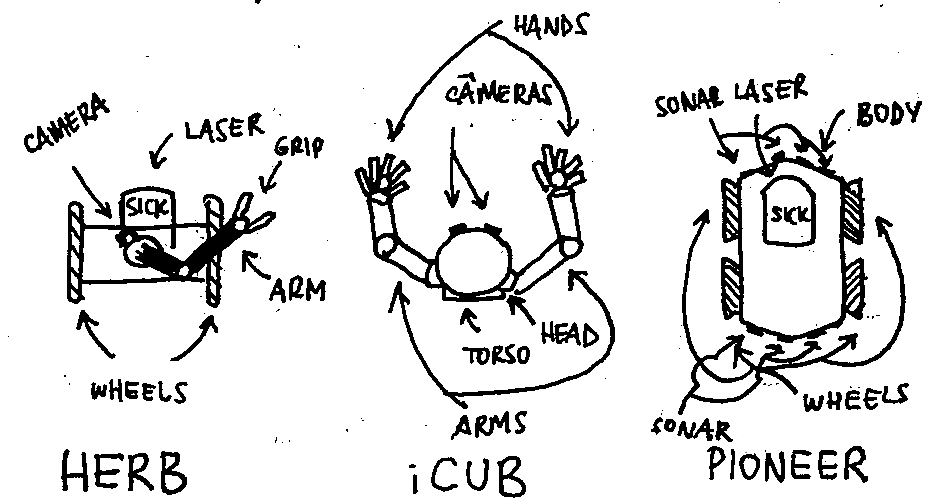
\includegraphics{figures/herb_icub_pioneer.png}
\caption{HERB, iCub, and Pioneer P3-DX robots}
\label{fig:herb_icub_pioneer}
\end{figure}

The HERB sees the world in \emph{forward mode} through its laser range finder
and its camera, coupled with its body movement. The iCub, in its
\emph{paraplegical} version, can only see the world in a left-to-right (and
right-to-left) manner through its cameras and head/torso movement. It can also
grasp nearby objects in order to examine them better. Finally, the Pioneer P3-DX
experiences the world in two different directions at the same time through its
sonars and its wheels movement. 

\bibliographystyle{plain}
\bibliography{prsurvey}

\end{document}
